% =====================================================================
%  Informe académico — Trabajo Práctico Grupal
%  Laboratorio de Métodos Cuantitativos Aplicados a la Gestión · FCE UBA
%  Compilar con pdfLaTeX (Overleaf o: latexmk -pdf -cd informe/main.tex)
% =====================================================================
\documentclass[10pt,a4paper]{article}

% ---------- Idioma y codificación ----------
\usepackage[utf8]{inputenc}
\usepackage[T1]{fontenc}
\usepackage[spanish,es-tabla,es-noshorthands]{babel}
\usepackage{lmodern}
\usepackage{microtype}

% ---------- Página ----------
\usepackage[a4paper,top=2.2cm,bottom=2.2cm,left=2.4cm,right=2.4cm]{geometry}
\usepackage{fancyhdr}
\usepackage{setspace}
\setstretch{1.05}
\setlength{\parskip}{0.35em}
\setlength{\parindent}{0pt}

% ---------- Tablas, figuras y color ----------
\usepackage{graphicx}
\graphicspath{{figuras/}}
\usepackage{booktabs}
\usepackage{array}
\usepackage{tabularx}
\usepackage{multirow}
\usepackage{float}
\usepackage{wrapfig}
\usepackage[font=small,labelfont=bf,skip=4pt]{caption}
\usepackage{subcaption}
\usepackage[table]{xcolor}
\definecolor{azul}{HTML}{2A78D6}
\definecolor{naranja}{HTML}{EB6834}
\definecolor{gristexto}{HTML}{555555}
\definecolor{fondocaja}{HTML}{F3F6FB}

% ---------- Listas y títulos ----------
\usepackage{enumitem}
\setlist{itemsep=2pt,topsep=3pt,leftmargin=1.4em}
\usepackage{titlesec}
\titleformat{\section}{\large\bfseries\color{azul!70!black}}{\thesection.}{0.5em}{}
\titleformat{\subsection}{\normalsize\bfseries}{\thesubsection.}{0.5em}{}
\titlespacing*{\section}{0pt}{1.0em}{0.4em}
\titlespacing*{\subsection}{0pt}{0.7em}{0.25em}

% ---------- Recuadro de hallazgo ----------
\usepackage[most]{tcolorbox}
\newtcolorbox{hallazgo}{colback=fondocaja,colframe=azul,boxrule=0pt,leftrule=2.5pt,
  arc=0pt,left=6pt,right=6pt,top=3pt,bottom=3pt,before skip=6pt,after skip=6pt}

% ---------- Enlaces ----------
\usepackage[hidelinks]{hyperref}
\usepackage{url}

% ---------- Encabezado y pie ----------
\pagestyle{fancy}
\fancyhf{}
\fancyhead[L]{\small\color{gristexto}Laboratorio de Métodos Cuantitativos · FCE UBA}
\fancyhead[R]{\small\color{gristexto}Impacto de las redes sociales en los estudiantes}
\fancyfoot[C]{\small\thepage}
\renewcommand{\headrulewidth}{0.4pt}

% ---------- Datos editables de la portada ----------
\newcommand{\repositorio}{\url{https://github.com/Chaile-Mendez/tp-analisis-labo}}
\newcommand{\overleaf}{[Link al proyecto de Overleaf]}

\begin{document}

% =====================================================================
% ---------------------------------------------------------------------
%  Portada  —  reemplazar los datos entre corchetes
% ---------------------------------------------------------------------
\begin{titlepage}
\thispagestyle{empty}
\centering
{\scshape Universidad de Buenos Aires · Facultad de Ciencias Económicas\par}
\vspace{0.15cm}
{\scshape\small Tecnicatura Universitaria en Gestión y Análisis de Datos en Organizaciones\par}
\vspace{0.15cm}
{\small Laboratorio de Métodos Cuantitativos Aplicados a la Gestión\par}

\vspace{2.6cm}
\rule{\linewidth}{0.6pt}\par
\vspace{0.5cm}
{\LARGE\bfseries Impacto de las redes sociales en los estudiantes\par}
\vspace{0.35cm}
{\large Uso diario, sueño, salud mental y rendimiento académico\\
según país, plataforma, género y situación sentimental\par}
\vspace{0.4cm}
\rule{\linewidth}{0.6pt}\par

\vspace{0.6cm}
{\large Trabajo Práctico Grupal — Informe académico\par}
\vspace{0.2cm}
{\normalsize 2.\textsuperscript{do} Cuatrimestre 2026\par}

\vspace{2.0cm}
{\bfseries Integrantes\par}
\vspace{0.3cm}
\renewcommand{\arraystretch}{1.35}
\begin{tabular}{l l l}
\toprule
\textbf{Nombre y apellido} & \textbf{N.º de registro} & \textbf{Usuario de GitHub} \\
\midrule
{[NOMBRE Y APELLIDO 1]} & {[REGISTRO 1]} & {[@usuario1]} \\
{[NOMBRE Y APELLIDO 2]} & {[REGISTRO 2]} & {[@usuario2]} \\
{[NOMBRE Y APELLIDO 3]} & {[REGISTRO 3]} & {[@usuario3]} \\
{[NOMBRE Y APELLIDO 4]} & {[REGISTRO 4]} & {[@usuario4]} \\
{[NOMBRE Y APELLIDO 5]} & {[REGISTRO 5]} & {[@usuario5]} \\
\bottomrule
\end{tabular}

\vfill
{\small\textbf{Repositorio:} \repositorio\par}
\vspace{0.1cm}
{\small\textbf{Proyecto Overleaf:} \overleaf\par}
\vspace{0.4cm}
{\small Buenos Aires, noviembre de 2026\par}
\end{titlepage}
\setcounter{page}{1}

% =====================================================================

% ---------------------------------------------------------------------
%  §1. Resumen
% ---------------------------------------------------------------------
\section*{Resumen}

Este informe analiza cómo se asocia el uso de redes sociales con el sueño, la salud mental y el rendimiento
académico percibido de 1.743 estudiantes de 18 a 24 años de 110 países. Mediante un análisis descriptivo
—comparación de medias, medianas y proporciones por grupo, correlaciones y visualizaciones— se evalúan el
nivel de desarrollo del país, la plataforma más usada, el género y la situación sentimental. El impacto no es
igual para todos: los estudiantes de países en desarrollo, quienes declaran que las redes afectan su
rendimiento y los usuarios de WhatsApp, TikTok y Snapchat presentan perfiles menos favorables. El factor
común es la \textbf{cantidad de horas de uso}, que se correlaciona negativamente con el sueño ($-0{,}79$) y
con la salud mental ($-0{,}82$); el género y la situación sentimental casi no muestran diferencias.

\noindent\textbf{Palabras clave:} redes sociales, estudiantes, salud mental, sueño, rendimiento académico.

% ---------------------------------------------------------------------
%  §2. Introducción
% ---------------------------------------------------------------------
\section{Introducción}

El uso de redes sociales forma parte de la vida cotidiana de los estudiantes, pero su impacto puede no ser
igual para todos. Hablar de “redes sociales” en general esconde que no todas se usan igual, y el contexto de
cada estudiante —el país en que vive, su género o su situación personal— puede influir en sus hábitos
digitales y en sus consecuencias. Identificar qué grupos y qué patrones de uso se asocian con peor
bienestar permite formular recomendaciones más específicas.

El trabajo utiliza el conjunto de datos \textit{Students Social Media Addiction}, publicado en Kaggle
\cite{kaggle}, con información de estudiantes secundarios, universitarios y de posgrado sobre su uso diario
de redes, la plataforma que más utilizan, sus horas de sueño, un puntaje de salud mental, su percepción
sobre si las redes afectan su rendimiento académico y su situación sentimental.

\begin{hallazgo}
\textbf{Pregunta principal:} \textit{¿cómo impacta el uso de redes sociales en los estudiantes y es ese
impacto igual para todos?} Se descompone en cuatro preguntas:
\begin{enumerate}[label=\arabic*.,itemsep=0pt,topsep=2pt]
  \item ¿El impacto es igual para todos los estudiantes según el nivel de desarrollo de su país?
  \item ¿El uso de redes sociales impacta en el sueño y en el rendimiento académico?
  \item ¿Hay redes sociales que impactan más que otras y existe una brecha de género en ese impacto?
  \item ¿El uso de redes sociales afecta las relaciones sentimentales de los estudiantes?
\end{enumerate}
\end{hallazgo}

En todo el informe, un puntaje de salud mental más alto representa un \textbf{mejor} estado de salud mental.

% ---------------------------------------------------------------------
%  §3. Datos y metodología
% ---------------------------------------------------------------------
\section{Datos y metodología}

\textbf{Estructura.} La base contiene \textbf{1.743 registros} y \textbf{11 variables} sobre estudiantes de
18 a 24 años de \textbf{110 países}, con una distribución de género pareja (883 varones y 860 mujeres). Las
variables centrales son el \textbf{uso diario de redes} (de 1,5 a 8,5 horas; media 4,98), las \textbf{horas
de sueño} por noche (de 3,8 a 9,6; media 6,78), el \textbf{puntaje de salud mental} (escala de 4 a 9, más
alto = mejor; media 6,21), el \textbf{impacto académico percibido} (si el estudiante \emph{declara} que las
redes afectan su rendimiento; es una percepción y no una medición de sus notas), la \textbf{plataforma más
usada} (12 redes, con Instagram, 550, y TikTok, 350, concentrando más de la mitad) y el \textbf{estado
sentimental} (soltero/a, en pareja o complicado), además de país, género, edad y nivel académico.

\textbf{Calidad de los datos.} No se detectaron valores atípicos, pero sí dos problemas relevantes. El
estado sentimental es la única variable incompleta, con 1.038 valores faltantes (59,55\,\%). Además,
\textbf{705 estudiantes} aparecían cargados dos veces —una sin estado sentimental y otra con ese dato—,
por lo que a simple vista parecían filas distintas. El identificador de estudiante tampoco es único: hay
números compartidos por personas diferentes (distinto género, país y edad), que se conservaron.

\textbf{Transformaciones.}
\begin{itemize}
  \item \textbf{Nivel de desarrollo del país:} según la clasificación por ingreso del Banco Mundial
  \cite{bancomundial}, las economías de ingreso alto se agruparon como \emph{Desarrollado} y el resto como
  \emph{En desarrollo} (1.103 y 638 estudiantes). Ciudad del Vaticano (2 registros) no figura en esa
  clasificación y quedó excluida de esta comparación.
  \item \textbf{Eliminación de duplicados:} para el análisis por plataforma y género se dejó una sola copia
  de cada estudiante repetido, con lo que la base quedó en \textbf{1.038 estudiantes}.
  \item \textbf{Plataformas minoritarias:} WeChat, LINE, KakaoTalk y VKontakte, con muy pocos casos, se
  agruparon en la categoría \emph{Otras} para evitar promedios inestables.
  \item \textbf{Niveles de uso:} \emph{Bajo} (hasta 4 h, 278 estudiantes), \emph{Medio} (entre 4 y 6 h,
  493) y \emph{Alto} (más de 6 h, 267), para comparar plataformas entre estudiantes con un uso similar.
  \item \textbf{Impacto académico como proporción:} la respuesta Sí/No se convirtió en un indicador cuyo
  promedio equivale al porcentaje de estudiantes que se sienten afectados.
\end{itemize}

Las preguntas 1 y 2 se analizan sobre los 1.743 registros (al repetir los cálculos principales sin
duplicados los resultados cambian solo en los decimales y las conclusiones se mantienen), la pregunta 3
sobre los 1.038 estudiantes sin duplicados y la pregunta 4 sobre los 705 registros con estado sentimental
completo.

\textbf{Enfoque y herramientas.} El análisis es \textbf{descriptivo}: se comparan medias, medianas y
proporciones entre grupos, se calculan correlaciones y rectas de tendencia, y se construyen histogramas,
diagramas de caja, gráficos de barras y de dispersión. El procesamiento se realizó en Python (pandas,
NumPy, Matplotlib y seaborn) en Google Colab \cite{mckinney}. Los resultados describen asociaciones dentro
de la muestra y no permiten establecer relaciones causales.

% ---------------------------------------------------------------------
%  §4. Resultados
% ---------------------------------------------------------------------
\section{Resultados}

% =====================================================================
\subsection{Nivel de desarrollo del país}

Los estudiantes de \textbf{países en desarrollo} muestran resultados menos favorables en los cuatro
indicadores (Tabla~\ref{tab:desarrollo}): usan más las redes (5,25 horas diarias contra 4,83), duermen
menos (6,45 horas contra 6,97), tienen un puntaje de salud mental más bajo (5,94 contra 6,37) y declaran con
mayor frecuencia que las redes afectan su rendimiento académico (74\,\% contra 56\,\%). La diferencia en el
descanso alcanza a toda la distribución (Figura~\ref{fig:sueno_desarrollo}): la mediana es de 6,3 horas
por noche contra 7,1, y la mitad central de cada grupo se ubica más abajo en los países en desarrollo
(entre 5,7 y 7,2 horas) que en los desarrollados (entre 6,1 y 7,8 horas), con una dispersión parecida.

\begin{table}[H]
\centering
\small
\caption{Indicadores según el nivel de desarrollo del país (media y mediana).}
\label{tab:desarrollo}
\begin{tabular}{l cc cc cc c}
\toprule
& \multicolumn{2}{c}{\textbf{Uso diario (h)}} & \multicolumn{2}{c}{\textbf{Sueño (h)}}
& \multicolumn{2}{c}{\textbf{Salud mental}} & \textbf{Afecta rend.} \\
\cmidrule(lr){2-3}\cmidrule(lr){4-5}\cmidrule(lr){6-7}\cmidrule(lr){8-8}
\textbf{Nivel de desarrollo} & Media & Mediana & Media & Mediana & Media & Mediana & \% Sí \\
\midrule
Desarrollado ($n=1.103$)  & 4,83 & 4,6 & 6,97 & 7,1 & 6,37 & 6,3 & 56,48 \\
En desarrollo ($n=638$)   & 5,25 & 5,2 & 6,45 & 6,3 & 5,94 & 6,0 & 74,45 \\
\bottomrule
\end{tabular}
\end{table}

% =====================================================================
\subsection{Uso de redes, sueño y rendimiento académico}

Se observa una clara relación negativa entre el uso de redes y el descanso (Figura~\ref{fig:uso_sueno}):
la correlación es de $\mathbf{-0{,}79}$ y, según la recta de tendencia, cada hora adicional de uso diario se
asocia en promedio con unas \textbf{0,65 horas menos de sueño}.

\begin{figure}[H]
\centering
\begin{subfigure}[t]{0.46\linewidth}
  \centering
  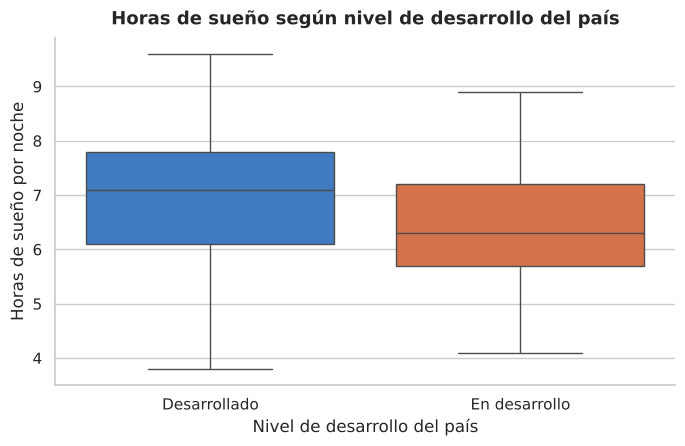
\includegraphics[width=\linewidth]{fig01_sueno_desarrollo.png}
  \caption{Según nivel de desarrollo del país.}
  \label{fig:sueno_desarrollo}
\end{subfigure}\hspace{0.03\linewidth}
\begin{subfigure}[t]{0.38\linewidth}
  \centering
  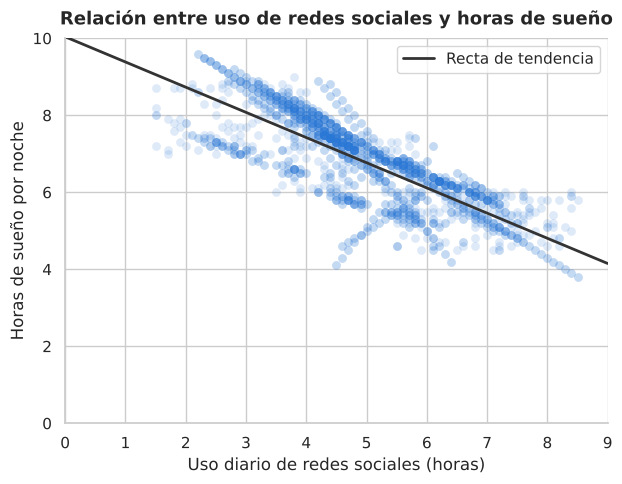
\includegraphics[width=\linewidth]{fig02_uso_sueno.png}
  \caption{Según uso diario de redes, con recta de tendencia.}
  \label{fig:uso_sueno}
\end{subfigure}
\caption{Horas de sueño por noche de los estudiantes.}
\label{fig:sueno}
\end{figure}

El 63\,\% de los estudiantes (1.100 de 1.743) declara que las redes afectan su rendimiento académico, y
quienes se sienten perjudicados se concentran en la zona de más horas de uso y menos horas de sueño
(Figura~\ref{fig:uso_sueno_impacto}). Este grupo usa las redes 1,7 horas más por día y duerme 1,4 horas
menos que el resto (Tabla~\ref{tab:academico}); las medianas son casi iguales a las medias, por lo que la
diferencia no se debe a unos pocos casos extremos. La brecha más marcada aparece en el descanso: \textbf{el
77\,\% de los que se sienten afectados duerme menos de 7 horas}, el mínimo recomendado para adultos
\cite{watson}, contra el 13\,\% del otro grupo.

\begin{figure}[H]
\centering
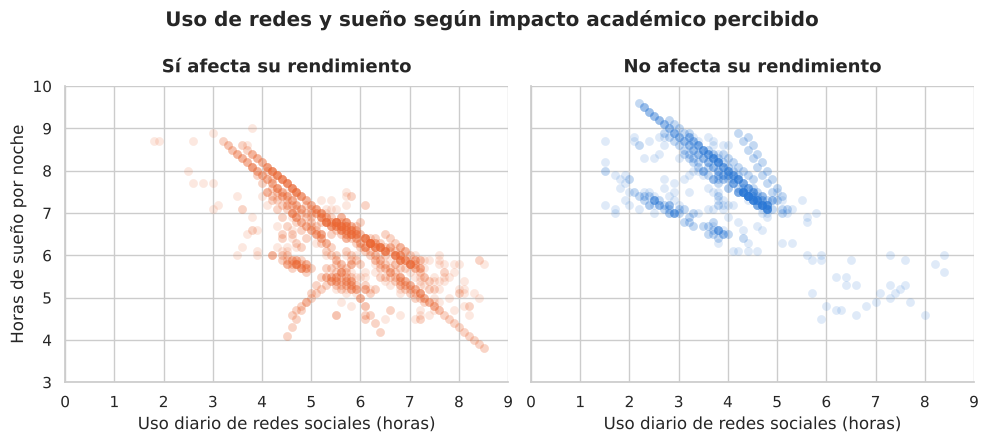
\includegraphics[width=0.60\linewidth]{fig03_uso_sueno_impacto.png}
\caption{Uso de redes y sueño según el impacto académico percibido.}
\label{fig:uso_sueno_impacto}
\end{figure}

\begin{table}[H]
\centering
\small
\caption{Uso y sueño según el impacto académico percibido.}
\label{tab:academico}
\begin{tabular}{l c cc cc c}
\toprule
\textbf{¿Las redes afectan} & & \multicolumn{2}{c}{\textbf{Uso diario (h)}} & \multicolumn{2}{c}{\textbf{Sueño (h)}} & \textbf{Duerme} \\
\cmidrule(lr){3-4}\cmidrule(lr){5-6}
\textbf{su rendimiento?} & \textbf{Estudiantes} & Media & Mediana & Media & Mediana & \textbf{< 7 h (\%)} \\
\midrule
No & 643   & 3,88 & 3,9 & 7,65 & 7,6 & 13,06 \\
Sí & 1.100 & 5,62 & 5,6 & 6,27 & 6,2 & 76,64 \\
\bottomrule
\end{tabular}
\end{table}

% =====================================================================
\subsection{Plataformas y brecha de género}

\textbf{Diferencias entre plataformas.} Sobre los 1.038 estudiantes sin duplicados se observan grandes
diferencias según la red más usada (Tabla~\ref{tab:plataforma}). \textbf{WhatsApp} muestra los resultados
más preocupantes: más horas de uso (6,5 h), menos sueño (5,9 h), la peor salud mental (5,54) y el
100\,\% de sus usuarios declara que las redes afectan su rendimiento. Le siguen \textbf{TikTok} (5,77) y
\textbf{Snapchat} (5,81). En el otro extremo, \emph{Otras} (6,84), \textbf{LinkedIn} (6,77),
\textbf{Twitter} (6,57) y \textbf{Facebook} (6,51) combinan mejor salud mental, más sueño y menor
afectación académica; Instagram, la más usada, queda en una posición intermedia (6,15).

\begin{table}[H]
\centering
\footnotesize
\setlength{\tabcolsep}{4pt}
\caption{Indicadores promedio según la plataforma más usada, ordenados de peor a mejor salud mental, y
salud mental promedio dentro de cada nivel de uso diario.}
\label{tab:plataforma}
\begin{tabular}{l ccccc ccc}
\toprule
& & & & & & \multicolumn{3}{c}{\textbf{Salud mental por nivel de uso}} \\
\cmidrule(lr){7-9}
\textbf{Plataforma} & \textbf{Uso (h)} & \textbf{Sueño (h)} & \textbf{Salud m.} & \textbf{Afecta} & \textbf{$n$}
& \textbf{Bajo ($\leq$4 h)} & \textbf{Medio (4--6 h)} & \textbf{Alto ($>$6 h)} \\
\midrule
WhatsApp  & 6,48 & 5,87 & 5,54 & 1,00 & 54  & --   & 5,82 & 5,41 \\
TikTok    & 5,38 & 6,32 & 5,77 & 0,85 & 196 & 7,11 & 5,89 & 4,87 \\
Snapchat  & 5,54 & 6,01 & 5,81 & 0,77 & 60  & 7,43 & 5,87 & 4,99 \\
Instagram & 4,88 & 6,96 & 6,15 & 0,65 & 301 & 7,42 & 6,04 & 4,72 \\
YouTube   & 4,91 & 6,51 & 6,34 & 0,52 & 65  & 7,46 & 5,98 & 5,09 \\
Facebook  & 4,83 & 7,08 & 6,51 & 0,41 & 172 & 7,64 & 6,63 & 4,86 \\
Twitter   & 4,89 & 6,67 & 6,57 & 0,51 & 73  & 7,49 & 6,72 & 5,05 \\
LinkedIn  & 4,23 & 6,82 & 6,77 & 0,33 & 66  & 7,82 & 6,17 & 4,64 \\
Otras     & 4,34 & 7,61 & 6,84 & 0,39 & 51  & 7,67 & 6,39 & --   \\
\midrule
\multicolumn{6}{l}{\textbf{Promedio de cada nivel de uso (todas las plataformas)}} & \textbf{7,51} & \textbf{6,16} & \textbf{4,93} \\
\bottomrule
\end{tabular}

\smallskip
{\footnotesize\textit{Nota:} “Afecta” es la proporción de estudiantes que declara que las redes afectan su
rendimiento (0,33 equivale al 33\,\%); $n$ es la cantidad de estudiantes; “--” indica que no hay
estudiantes en esa combinación.}
\end{table}

En la Figura~\ref{fig:uso_salud_plataforma} cada punto es una plataforma y los puntos bajan de izquierda
a derecha: \textbf{cuantas más horas de uso promedio tiene una plataforma, menor es la salud mental promedio
de sus usuarios}. WhatsApp acumula más horas y el peor puntaje; LinkedIn y \emph{Otras}, el menor uso
(alrededor de 4,3 h) y los mejores puntajes. Una hipótesis es que las plataformas de uso constante y alta
frecuencia se asocian con más horas de pantalla, y las de uso puntual con menos.

\begin{figure}[H]
\centering
\begin{subfigure}[t]{0.46\linewidth}
  \centering
  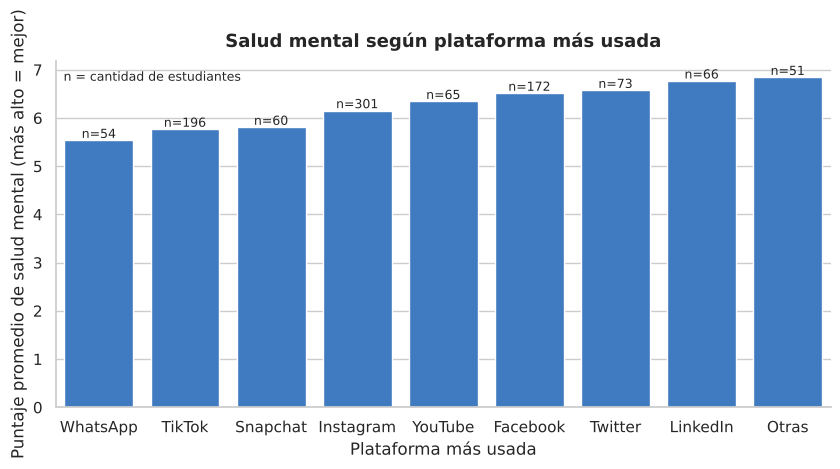
\includegraphics[width=\linewidth]{fig05_salud_plataforma.png}
  \caption{Salud mental promedio por plataforma.}
  \label{fig:salud_plataforma}
\end{subfigure}\hspace{0.03\linewidth}
\begin{subfigure}[t]{0.42\linewidth}
  \centering
  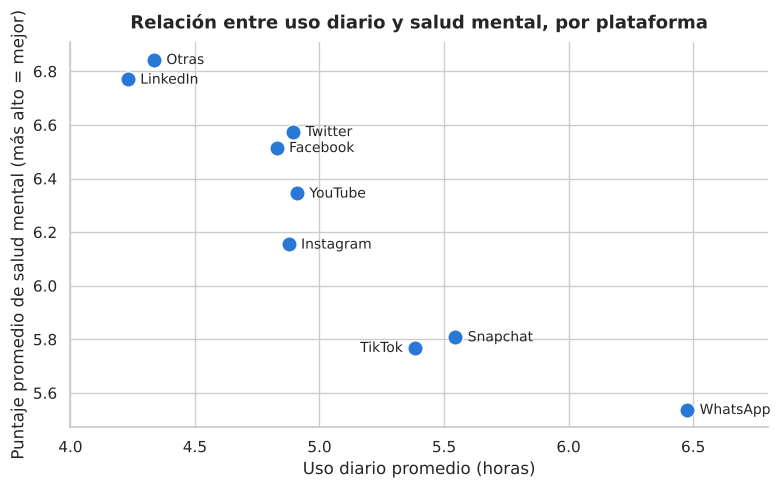
\includegraphics[width=\linewidth]{fig06_uso_salud_plataforma.png}
  \caption{Uso diario y salud mental promedio, por plataforma.}
  \label{fig:uso_salud_plataforma}
\end{subfigure}
\caption{Salud mental según la plataforma más usada.}
\label{fig:plataformas}
\end{figure}

\textbf{¿Es la plataforma o son las horas?} A nivel general, cuantas más horas se usan las redes, peor es
la salud mental (correlación de $-0{,}82$): el puntaje baja de 7,51 en el uso bajo a 6,16 en el medio y a
4,93 en el alto. Al comparar estudiantes con una cantidad de horas parecida (columnas derechas de la
Tabla~\ref{tab:plataforma}), las diferencias entre plataformas se achican de 1,3 puntos a entre 0,7 y 0,9:
\textbf{gran parte de la diferencia entre plataformas se debe a las horas de uso y no a la plataforma en
sí}. Aun así, en los niveles bajo y medio la diferencia no desaparece: entre quienes usan las redes de 4 a 6
horas, TikTok (5,89) y Snapchat (5,87) siguen por debajo de Facebook (6,63) y Twitter (6,72). Con un uso muy
intensivo, en cambio, el orden se mezcla: Facebook (4,86) queda a la par de TikTok (4,87), WhatsApp pasa a
tener el mejor promedio (5,41) y LinkedIn el peor (4,64). Las diferencias que persisten pueden deberse a la
plataforma o a que quienes la eligen sean distintos; con estos datos no es posible distinguirlo.

\begin{wrapfigure}{r}{0.42\linewidth}
\vspace{-1.2em}
\centering
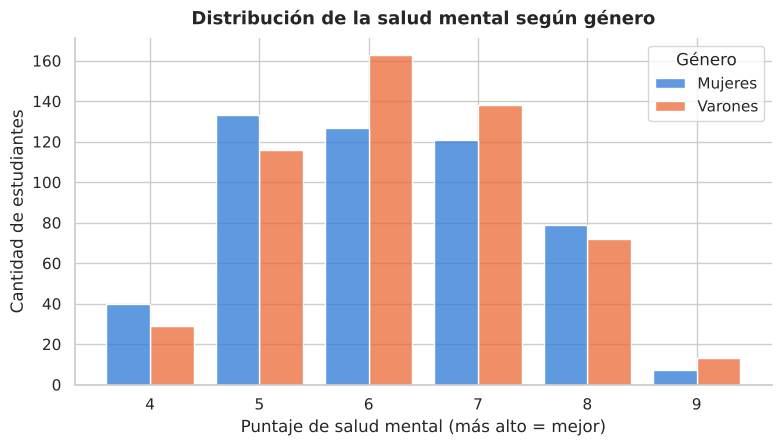
\includegraphics[width=\linewidth]{fig04_salud_genero.png}
\caption{Distribución del puntaje de salud mental según género.}
\label{fig:genero}
\vspace{-1em}
\end{wrapfigure}

\textbf{Brecha de género.} Las diferencias por género son muy chicas: mujeres y varones usan las redes
alrededor de 5 horas por día (5,08 contra 4,96), duermen cerca de 6,7 horas (6,68 contra 6,76) y la
afectación académica es casi idéntica (63\,\% contra 62\,\%). En salud mental los varones promedian 6,25 y
las mujeres 6,15, una diferencia de \textbf{0,10 puntos} con la misma mediana (6,0); ambas distribuciones
van del mismo mínimo al mismo máximo y concentran la mayoría de los casos entre 5 y 7
(Figura~\ref{fig:genero}). Dentro de cada plataforma las brechas también son chicas (0,42 puntos o menos,
la mayor en Snapchat, con pocos estudiantes) y \textbf{cambian de signo}: en Instagram, Twitter y
\emph{Otras} las mujeres tienen un puntaje levemente mayor, y en Snapchat, WhatsApp y Facebook, los
varones. La diferencia de género aparece, en cambio, en \emph{quién} usa cada red: Instagram es
mayoritariamente femenina (193 mujeres y 108 varones), mientras que Facebook (120 varones y 52 mujeres) y
WhatsApp (43 varones y 11 mujeres) son mayoritariamente masculinas. Por lo tanto, el género no explica que
unas plataformas se asocien con mejor o peor salud mental que otras.

% =====================================================================
\subsection{Relaciones sentimentales}

Entre los 705 estudiantes con estado sentimental informado, 384 están solteros, 289 en pareja y 32 en
una situación complicada. La media y la mediana del uso diario son muy parecidas en los tres grupos, entre
4,7 y 4,9 horas por día (Figura~\ref{fig:uso_estado}), por lo que no se observa una diferencia en la
cantidad de uso según la situación sentimental. La diferencia aparece en \emph{qué} plataforma se usa.
Como varias redes tienen pocas observaciones con este dato, la comparación se concentra en las tres más
usadas: Instagram (249), TikTok (154) y Facebook (123). La proporción de solteros es mayor en
\textbf{TikTok (65,6\,\%)} y en \textbf{Instagram (58,2\,\%)}, mientras que en \textbf{Facebook} la mayoría
está en pareja (57,7\,\%) (Figura~\ref{fig:estado_top3}). Las situaciones complicadas son algo más
frecuentes en TikTok (5,2\,\%) e Instagram (4,0\,\%) que en Facebook (0,8\,\%), aunque se trata de muy pocos
estudiantes (8, 10 y 1), por lo que esa diferencia es poco confiable.

\begin{figure}[H]
\centering
\begin{subfigure}[t]{0.46\linewidth}
  \centering
  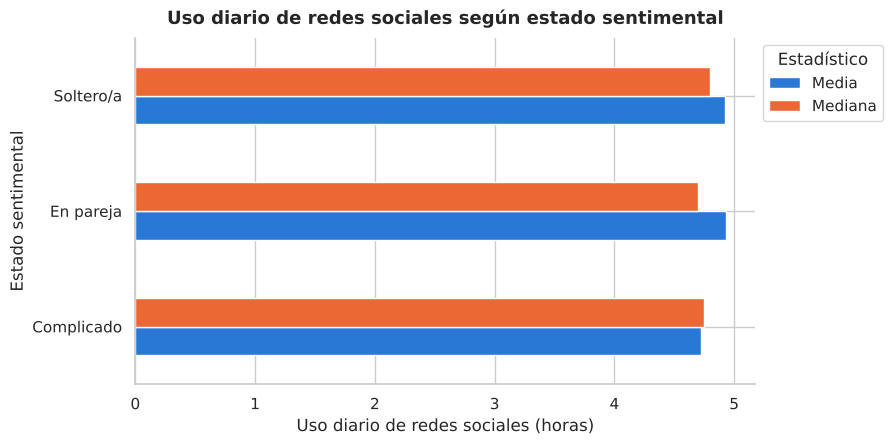
\includegraphics[width=\linewidth]{fig07_uso_estado_sentimental.png}
  \caption{Uso diario (media y mediana) según estado sentimental.}
  \label{fig:uso_estado}
\end{subfigure}\hspace{0.03\linewidth}
\begin{subfigure}[t]{0.44\linewidth}
  \centering
  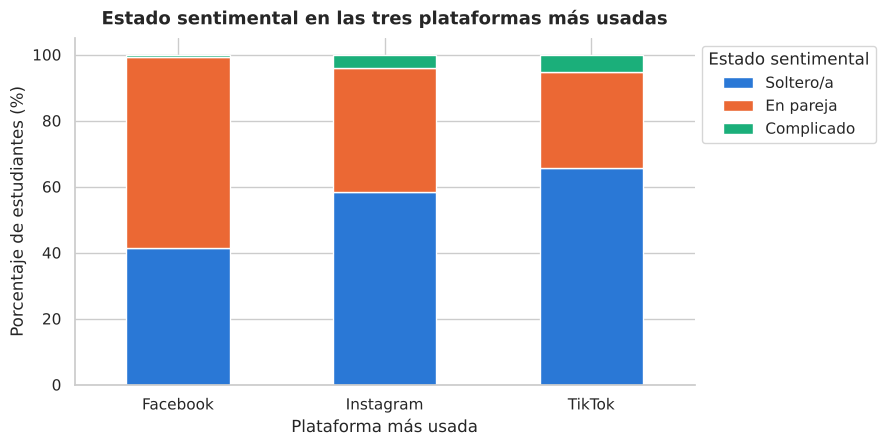
\includegraphics[width=\linewidth]{fig08_estado_top3.png}
  \caption{Estado sentimental en las tres plataformas más usadas.}
  \label{fig:estado_top3}
\end{subfigure}
\caption{Uso de redes sociales y situación sentimental.}
\label{fig:sentimental}
\end{figure}

% ---------------------------------------------------------------------
%  §5. Conclusiones
% ---------------------------------------------------------------------
\section{Conclusiones}

\begin{enumerate}[label=\arabic*.]
  \item \textbf{Nivel de desarrollo:} el impacto no es igual para todos. Los estudiantes de países en
  desarrollo presentan más horas de uso, menos sueño, peor salud mental y mayor afectación académica percibida.
  \item \textbf{Sueño y rendimiento:} a mayor uso, menos sueño. Tres de cada cuatro estudiantes que se sienten
  afectados académicamente duermen menos de 7 horas, contra uno de cada ocho entre quienes no. Esto es
  coherente con que parte del impacto académico se dé a través de la falta de sueño, aunque el análisis no
  permite confirmarlo.
  \item \textbf{Plataformas y género:} WhatsApp, TikTok y Snapchat se asocian con peores resultados, y
  LinkedIn, Twitter y Facebook con resultados más favorables, pero gran parte de la diferencia se explica por
  las horas de uso. La brecha de género es muy leve.
  \item \textbf{Relaciones sentimentales:} el uso diario es prácticamente igual entre solteros, en pareja y en
  situación complicada; las diferencias en la plataforma elegida describen el perfil de sus usuarios, no un
  efecto de la red sobre las relaciones.
\end{enumerate}

\begin{hallazgo}
\textbf{Conclusión general.} Las cuatro preguntas convergen en un mismo patrón: \textbf{la cantidad de horas
de uso es el factor que más se repite detrás de los resultados menos favorables}. Los grupos con peores
indicadores son también los que más horas pasan en las redes, y a más horas se observan menos sueño y menor
salud mental. Más que \emph{qué} red se usa o \emph{quién} la usa, el dato más útil para anticipar un impacto
negativo es \textbf{cuánto tiempo se le dedica}.
\end{hallazgo}

\textbf{Limitaciones.} Los resultados son descriptivos y no permiten establecer causalidad; el rendimiento
académico es autodeclarado y no una medición de las notas; la clasificación por desarrollo se basa solo en el
ingreso y los grupos están desbalanceados (1.103 contra 638); varias plataformas tienen pocos casos y el estado
sentimental falta en el 59,55\,\% de los registros; y las preguntas 1 y 2 incluyen los 705 registros
duplicados, aunque sin ellos las conclusiones se mantienen.

\textbf{Extensiones.} Para confirmar la relación haría falta un estudio que siga a los mismos estudiantes a lo
largo del tiempo y mida el rendimiento académico con datos objetivos, en lugar de la percepción de cada
estudiante.

% ---------------------------------------------------------------------
%  §6. Reflexión metodológica
% ---------------------------------------------------------------------
\section{Reflexión metodológica}

\textbf{Uso de IA.} La IA se utilizó como asistente para sugerir transformaciones y gráficos, revisar la
redacción de las interpretaciones y redactar este informe en \LaTeX{} a partir del notebook ejecutado, con
una instrucción de rol de analista de datos que exigía usar exactamente sus números, gráficos y conclusiones.
La interpretación y las decisiones de análisis fueron responsabilidad del grupo.
\textbf{Revisiones.} Cada integrante contrastó las afirmaciones del informe con el notebook y los datos
originales, y el grupo consolidó los comentarios. [COMPLETAR: comentarios de la validación externa y cómo se
incorporaron.]
\textbf{Aprendizajes.} Auditar la calidad de los datos es indispensable: la verificación estándar no detectaba
filas repetidas, y solo al notar que el identificador máximo (1.000) era menor que la cantidad de filas
(1.743) se descubrieron 705 estudiantes cargados dos veces. También se comprobó que una diferencia entre
grupos puede deberse a una tercera variable —las horas de uso—, lo que cambió la lectura de las diferencias
entre plataformas.

% ---------------------------------------------------------------------
%  §7. Bibliografía
% ---------------------------------------------------------------------
\begin{thebibliography}{9}
\small

\bibitem{kaggle}
Shamim, A. (2025). \textit{Students' Social Media Addiction} [Conjunto de datos]. Kaggle.
\url{https://www.kaggle.com/datasets/adilshamim8/social-media-addiction-vs-relationships}

\bibitem{bancomundial}
Banco Mundial (2025). \textit{World Bank Country and Lending Groups}. Clasificación de economías por
nivel de ingreso.
\url{https://datahelpdesk.worldbank.org/knowledgebase/articles/906519-world-bank-country-and-lending-groups}

\bibitem{watson}
Watson, N. F., Badr, M. S., Belenky, G., et al. (2015). Recommended amount of sleep for a healthy adult:
A joint consensus statement of the American Academy of Sleep Medicine and Sleep Research Society.
\textit{Sleep}, 38(6), 843--844.

\bibitem{mckinney}
McKinney, W. (2010). Data structures for statistical computing in Python. \textit{Proceedings of the 9th
Python in Science Conference}, 56--61.

\end{thebibliography}


\end{document}
